\begin{frame}{KNOWLEDGE DISTILLATION}
    \begin{figure}
        \centering
        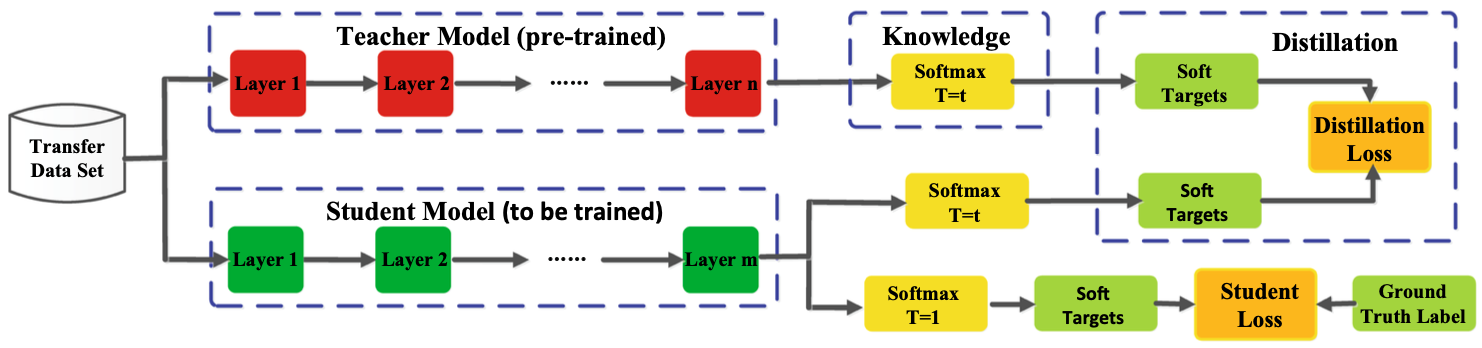
\includegraphics[width = 0.9\linewidth]{KD_losses.png}
        \centering
        \caption{Generazione cross-entropy $L_{soft}$ (in alto) e $L_{hard}$ (in basso).}
        \label{l_hard_soft}
    \end{figure}
    \vspace{-0.3cm}
     Applicata principalmente per task di \emph{image classification}, ha l'obiettivo di addestrare un modello \emph{"Studente"} grazie all conoscenza distillata trasferita da un modello \emph{"Insegnante"}.
     \begin{minipage}{\linewidth}
        \centering
        \begin{minipage}{0.45\linewidth}
            Elementi chiave:
            \begin{itemize}
                \item {\bfseries{\emph{Temperatura $T$}}};
                \item {\bfseries{\emph{Soft-targets}}};
                \item {\bfseries{\emph{Perdita complessiva}}}.
            \end{itemize}
        \end{minipage}
        \begin{minipage}{0.40\linewidth}
            \begin{block}{\centering Soft-targets}
                \centering
                $ q_j = \frac{e^{z_j/T}}{\sum_{k=1}^K e^{z_k/T}} $
            \end{block} 
            \begin{block}{\centering Total Loss}
                \centering \small $ L= L_{hard}+T^2L_{soft} $
            \end{block}
        \end{minipage}
    \end{minipage}
\end{frame}